
%%%%%%%%%%%%%%%%%%%%%%% file typeinst.tex %%%%%%%%%%%%%%%%%%%%%%%%%
%
% This is the LaTeX source for the instructions to authors using
% the LaTeX document class 'llncs.cls' for contributions to
% the Lecture Notes in Computer Sciences series.
% http://www.springer.com/lncs       Springer Heidelberg 2006/05/04
%
% It may be used as a template for your own input - copy it
% to a new file with a new name and use it as the basis
% for your article.
%
% NB: the document class 'llncs' has its own and detailed documentation, see
% ftp://ftp.springer.de/data/pubftp/pub/tex/latex/llncs/latex2e/llncsdoc.pdf
%
%%%%%%%%%%%%%%%%%%%%%%%%%%%%%%%%%%%%%%%%%%%%%%%%%%%%%%%%%%%%%%%%%%%


\documentclass[runningheads,a4paper]{llncs}

\usepackage{amssymb}
\setcounter{tocdepth}{3}
\usepackage{subcaption}
\usepackage{graphicx}
\usepackage{natbib}
\usepackage{enumitem}
\usepackage[options ]{algorithm2e}

\usepackage{url}
\urldef{\mailsa}\path|nitin.nilesh@research.iiit.ac.in, jawahar.iiit.ac.in|  
\newcommand{\keywords}[1]{\par\addvspace\baselineskip
\noindent\keywordname\enspace\ignorespaces#1}

\begin{document}

\mainmatter  % start of an individual contribution

% first the title is needed
\title{Structured Real-Time Analysis of Live Badminton Game}

% a short form should be given in case it is too long for the running head
%\titlerunning{Lecture Notes in Computer Science: Authors' Instructions}

% the name(s) of the author(s) follow(s) next
%
% NB: Chinese authors should write their first names(s) in front of
% their surnames. This ensures that the names appear correctly in
% the running heads and the author index.
%
\author{Nitin Nilesh, C. V. Jawahar}
%
\authorrunning{Structured Real-Time Analysis of Live Badminton Game}
% (feature abused for this document to repeat the title also on left hand pages)

% the affiliations are given next; don't give your e-mail address
% unless you accept that it will be published
\institute{Centre for Visual Information Technology,\\International Institute of Information Technology,\\
Hyderabad, India.\\
\mailsa\\
\mailsb\\
\mailsc\\}

%
% NB: a more complex sample for affiliations and the mapping to the
% corresponding authors can be found in the file "llncs.dem"
% (search for the string "\mainmatter" where a contribution starts).
% "llncs.dem" accompanies the document class "llncs.cls".
%

%\toctitle{Lecture Notes in Computer Science}
%\tocauthor{Authors' Instructions}
\maketitle


\begin{abstract}
\emph{Sports analysis is one of the major tasks in computer vision community for a long time and researchers from all over the world are focusing on this area. Analysis such as event prediction, object tracking, video summarization, highlight generation, etc. has been done in the past. However, all this analysis has been done on recorded videos after the match is over. In this work, we propose an end-to-end framework for Badminton game analysis done on live broadcast match videos.\\
We propose a method to calculate the distance covered by both the players during the game of Badminton on the live broadcast match by segmenting the points played, tracking and identifying the player into each point and finally calculating the distance of each player. We performed these analyses on live broadcast matches of Premier Badminton League - 2019 and shown the data live calculated using our method.}
\end{abstract}


\section{Introduction}

Sports analytics has been a major interest of computer
vision community for a long time. Applications of sport analytic system includes video summarization, event prediction \cite{giancola2018soccernet}, object detection \cite{maksai2016players}, structured analysis of the game \cite{ghosh2018towards}, fine-grained descriptions \cite{sukhwani2015tennisvid2text, sharma2015fine}, etc. Computer vision is also used behind-the-scenes, in areas such as training and coaching, and providing help for the referee during a game. Other current research topics include analysis of how groups of players move \cite{felsen2017will}, for applications like coaching in team sports, or automatically identifying key stages \cite{sharma2017automatic} in a game for gathering statistics or automating the control of broadcast cameras. Game statistics are important to show details of sports events. In badminton, games statistics consist of each player’s number of winners, unforced errors, successful smashes, and so on. They help coaches to design the strategy to improve their player’s performance. For viewers, game statistics would improve accessing the point of interest of a game. Sports videos, intended for live viewing, are commonly available for consumption in the form of broadcast videos. Today, there are several thousand hours worth of broadcast videos available on the web. Sport broadcast videos are often long and captured in the wild setting from multiple viewpoints. Additionally, these videos are usually edited and overlayed with animations or graphics. Automatic understanding of broadcast videos is difficult due to its `unstructured' nature coupled with the fast changing appearance and complex human pose and motion. These challenges have limited the scope of various existing sports analytics methods.

\subsection{Underlying Techniques}

In order to improve performance of athlete effectively, the coaching skill relies heavily on performance analysis. In badminton matches and in training, in order to select the tactics required to deal with different opponents, the  coach  must have a good statistical knowledge of the tactics of the player. Several studies have been performed to analyze the movement of players and the ball in sporting events, and many developments have been made in the past few years. The ultimate goal of this work was to develop a system capable of real-time statistical analysis of data collected during match-play, to  provide information to assist training and to select match tactics. Even today these analysis of sports videos is either done by human sports experts \cite{Dartfish} which is expensive and time consuming or rely on special camera setup \cite{reno2017technology} or additional sensors \cite{mlakar2017analyzing} which adds to the cost as well as limits their utility. With the recent improvement of computer hardware and technology related to image processing, computer vision is increasingly expected to replace manual operations in sports matches and training. \par
Deep learning based techniques have enabled a significant rise in the performance of various tasks such as object detection and recognition \cite{he2016deep, redmon2016you, ren2015faster, simonyan2014very}, action recognition \cite{wang2015action}, and temporal segmentation \cite{lea2016temporal, singh2016first}. Despite these advancements, recent attempts in sports analytics are not fully automatic for finer details \cite{chu2017badminton, yan2014automatic} or have a human in the loop for high level understanding of the game \cite{Dartfish, chu2017badminton} and, therefore, have limited practical applications to large scale data analysis.

\subsection{Contribution}

In  this  work,  we  aim  to  perform  automatic  annotation and provide informative analytics of sports broadcast videos, in particular, badminton games (refer to figure 1). We detect points (rally and non-rally) and players in each frame of the match to enable fast indexing and efficient retrieval. We, further, use these fine annotations to compute understandable metrics  (e.g.,  player’s  distance travelled,  heat-map of the players,  positioning and footwork around the court, etc.) for higher level analysis. \par
Badminton is the fastest racket game [13], and this makes playing pattern and speed different from other racket games. Similar to many other sports, badminton has specific game grammar (turn-based strokes, winning points, etc.), well separated playing areas (courts), structured as a series of events (points, rallies, and winning points), and therefore, are suited well for performing analytics at a very large scale. There are several benefits of such systems. Quantitative scores summarizes player's performance while qualitative game analysis enriches viewing experience. Player's strategy, strengths, and weaknesses could be mined and easily highlighted for training. It automates several aspects of analysis traditionally done manually by experts and coaches. \par 
\begin{figure}[h]
\centering
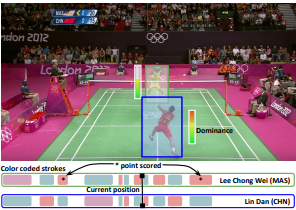
\includegraphics[width=0.9\textwidth]{Images/intro.png}
\caption{\label{fig:intro}We aim to automatically detect players, their tracks, points and distance covered by them in live broadcast videos of badminton games. This enables rich and informative analysis (reaction time, dominance, positioning, etc.) of each player at point as well as match level.}
\end{figure}

Badminton poses different difficulties for its automatic analysis. The actions (or  strokes) are  intermittent, fast-paced, have complex movements, and sometimes occluded by the other player.  Further, the best players employ various subtle deception strategies to fool the human opponent. The task becomes even more difficult with unstructured broadcast videos. The cameras have an oblique or overhead view of players and certain crucial aspects such as wrist and leg movements of both players may not be visible in the same frame. Tracking players across different views makes the problem even more complicated. We discard the highlights and process only clips from behind the baseline views which focus on both players and have minimal camera movements. For both points classification (rally/non-rally) and players detection, we rely on robust deep learning detection techniques. \par
The major contributions of this work are:

\begin{enumerate}[topsep=8pt,itemsep=4pt,partopsep=4pt, parsep=4pt]
    \item We propose an end-to-end framework to automatically annotate live badminton broadcast videos. Unlike previous approaches, our method does not rely on special camera setup or additional sensors.
    
    \item Using recent  advancements in object detection and temporal segmentation, we predict game points and its outcome, players' heatmap as well as their distance travelled across the gameplay.
    
    \item We introduce a live broadcast match videos based analysis technique with match level point segments and outcomes as well as frame level players' tracks. We us the official live broadcast videos of matches played in Premier Badminton League 2019.
\end{enumerate}

\section{Related Work}

\subsection{Sports Understanding and Applications}
Sports video analysis is an active research area. Traditional work in computer vision analyzing sports videos \cite{beetz2009aspogamo} has focused on either tracking players \cite{shitrit2011tracking} or balls \cite{maksai2016players}. Another body of work assumes the annotations of ball or player tracks to analyze game formations or skill level of individual players. A large body of work has focused on action recognition \cite{simonyan2014two, soomro2012ucf101, laptev2008learning}, people and object tracking \cite{urtasun20063d, weng2006video}. Several researchers have worked on improving sports understanding using domain specific cues in the past \cite{chen2014play, sha2014understanding}. Racket sports have received a lot of attention in this area with strides made in video summarization and highlight generation \cite{ghanem2012context} and generating text descriptions \cite{sukhwani2015tennisvid2text}. Reno et al. \cite{reno2017technology} proposed a platform for tennis which extract 3D ball trajectories using a specialized camera setup. Yoshikawa et al. \cite{yoshikawa2010automated} performed serve scene detection for badminton games with a specialized overhead camera setup. Chu et al. \cite{chu2017badminton} performed semi-automatic badminton video analysis by detecting the court and players, classifying strokes and clustering player strategy into offensive or defensive. Mlakar et al. \cite{mlakar2017analyzing} performed shot classification while Bertasius et al. \cite{bertasius2017baller} assessed a basketball player’s performance using videos from wearable devices. Chen and Wang \cite{chen2007statistical} proposed a method based on 2-D seriate images to discover statistics of a badminton match. Careelmont \cite{careelmont2013badminton} conducted badminton shot classification in compressed videos. The shuttlecock was detected and the stroke type was recognized based on the shuttlecock trajectory. Dierickx \cite{dierickx2014badminton} continued Careelmont’s work and improved performance of the trajectory extractor significantly. Overall, these works focus on shuttlecock trajectory extraction in order to facilitate classification. Unlike these approaches, our method does not rely on human inputs, special camera setup or additional sensors. Similar to our case, Sukhwani et al. \cite{sukhwani2016frame} and Ghosh et al. \cite{ghosh2017smart} computed frame level annotations in broadcast tennis videos, however, where Sukhwani et al. used a dictionary learning method to co-cluster available textual descriptions and Ghosh et al. used the scoreboard extraction approach to perform the index based analysis.\par
Our work is inspired by the work of \cite{ghosh2018towards} that proposes an end-to-end framework to automatically annotate badminton broadcast videos. Their work identify various understandable metrics, computed using the framework, for match and player analysis as well as qualitative understanding of badminton games.

\subsection{Point Segmentation}

To remove the highlights of the badminton game play i.e. classifying only rally parts of the game, histogram of oriented gradients together with support vector machine approach \cite{ghosh2018towards} has been used.
\subsection{Player Detection and Tracking}
An exhaustive survey of this area can be found in \cite{nguyen2012human}. Specific methods for sports videos \cite{mentzelopoulos2013active, yan2014automatic} and especially for handling occlusions \cite{held2016learning} have also been proposed in the past. In the context of applications involving player tracking data, Wang et al. \cite{wang2016classifying} used tracking data of basketball matches to perform offensive playcall classification while Cervone et al. \cite{cervone2014pointwise} did point-wise predictions and discussed defensive metrics.

\section{Badminton BWF Dataset}

We work on a collection of 31 badminton match videos
taken from the official Badminton World Federation channel on YouTube\footnote{https://www.youtube.com/user/bwf}. We focus on "singles" matches played between two players for two or three sets and are typically around an hour long. We have specially focused on three main players named "Saina Nehwal", "Pusarla V. Sindhu" and "Kidambi Srikanth". Statistics of the proposed dataset used in our experiments are provided in Table \ref{tab:dataset}
% Please add the following required packages to your document preamble:
% \usepackage{graphicx}
\begin{table}[]
\centering
\resizebox{0.7\textwidth}{!}{%
\begin{tabular}{|l|c|c|c|c|}
\hline
\textbf{Component} & \multicolumn{1}{l|}{\textbf{Classes}} & \multicolumn{1}{l|}{\textbf{Total}} & \multicolumn{1}{l|}{\textbf{Train}} & \multicolumn{1}{l|}{\textbf{Test}} \\ \hline
Matches            & NA                                    & 10                                  & 7                                   & 3                                  \\ \hline
Players            & NA                                    & 13                                  & 9                                   & 4                                  \\ \hline
Players bboxes     & 2                                     & 2986                                & 2153                                & 833                                \\ \hline
Point Segments     & 2                                     & 23156                               & \multicolumn{1}{l|}{15147}          & \multicolumn{1}{l|}{8009}          \\ \hline
\end{tabular}%
}
\caption{Various statistics of our Badminton BWF Dataset. Each match is typically one hour long. Train and test columns represents number of annotations used in respective split for experiments.}
\label{tab:dataset}
\end{table}

\subsection{Matches}

To train and validate our approach, we manually annotate a subset of 10 matches including all three players with equal distribution. For this, we select matches such that we cover all versatility of court structures and all opponents are unique for our three main players. We choose this criteria to incorporate maximum gameplay variations in our dataset as well as to avoid overfitting to any specific player for any of the tasks. We divide the 10 matches into training set of 7 matches and a test set of 3 matches. Note that this setup is identical to leave-N-subjects-out criteria which is followed in various temporal segmentation tasks \cite{fathi2011learning, singh2016first, stein2013combining}. Evaluation across pairs of unseen players also emphasize the generality of our approach.

\subsection{Players Bounding Boxes}

We focus on "singles" badminton matches of two players. The players switch court after each set and midway between the final set. In a common broadcast viewpoint one player plays in the court near to the camera while the other player in the distant court (see Fig.\ref{fig:intro}), which we refer to as bottom and top player respectively. We randomly sample and annotate 150 frames with bounding boxes for both players in each match (total around 3000 boxes) and use this for the player detection task. The players are occasionally mired by occlusion and the large playing area induces sudden fast player movements. As the game is very fast-paced, large pose and scale variations exist along with severe motion blur for both players.

\subsection{Strokes}

The badminton strokes can be broadly categorized as "serve", "forehand", "backhand", "lob", and "smash" (refer to Figure \ref{fig:shots} for representative images). Apart from this we identify one more class, "react" for the purpose of player’s gameplay analysis. A player can only perform one of five standard strokes when the shuttle is in his/her court while the opponent player waits and prepare for response stroke. After each stroke the time gap for response from other player is labeled as "react". Also, we differentiate between the stroke classes of the top player and the bottom player to identify two classes per stroke (say, "smash-top" and “smash-bottom”). We also add a "none" class for segments when there is no specific action occurring.

The "react" class is an important and unique aspect of our dataset. When a player plays aggressively, that allows very short duration for the opponent to decide and react. It is considered to be advantageous for the player as the opponent often fails to react in time or make a mistake in this short critical time. This aspect is evident in racket sports as a player plays only a single stroke (in a well separated playing space) at a time.
\begin{figure}[!htbp]
    \centering
    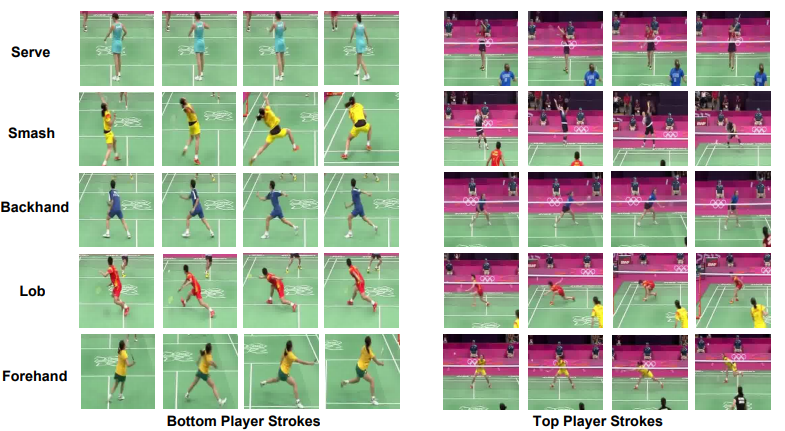
\includegraphics[width=0.9\linewidth]{Images/shots.png}
    \caption{Representative "strokes" of bottom and top players for each class defined.}
    \label{fig:shots}
\end{figure}

\section{Methodology}

\hspace{1cm}We start by finding the video segments that correspond to the play in badminton, discarding replays and other nonrelevant sections. We then proceed to detect, track and identify players across these play segments. Lastly, we calculate the distance covered by the players in each play segment. We use these predictions to generate a set of statistics for effective analysis of game play.

\subsection{Point Segmentation}

We segment out badminton "points" from the match by observing that usually the camera is behind the baseline during the play and involves minimal camera panning. Other camera views are discarded by our setup.  The replays are usually recorded from a closer angle and focus more on the drama of the stroke rather than the game in itself (however, rarely, points are also recorded from this view), and thus adds little or no extra information for further analysis.

We employ a convolutional neural network based approach to perform point segmentation task. We take every $10^{th}$ frame of the video and train a ResNet-18 \cite{he2016deep} based convolutional neural network to label the frame as a "point frame" or "non-point frame". We use this learned classifier to label each frame of the dataset as a "point frame" or otherwise. We are assuming that a rally is atleast 3 seconds long and use this parameter to group the frames into match rallies.

\begin{figure}[h]
    \centering
    \begin{subfigure}{\linewidth}
        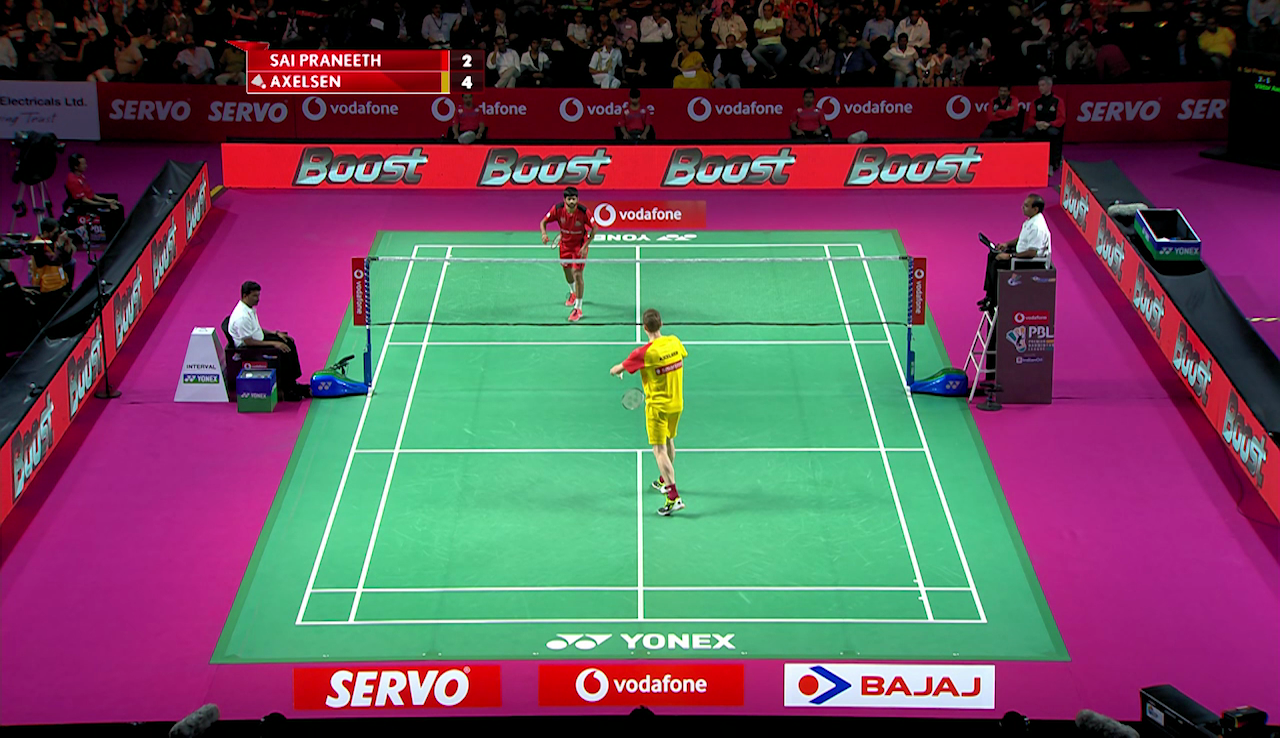
\includegraphics[width=.25\linewidth, height=.2\linewidth]{Images/rally1.png}\hfill
        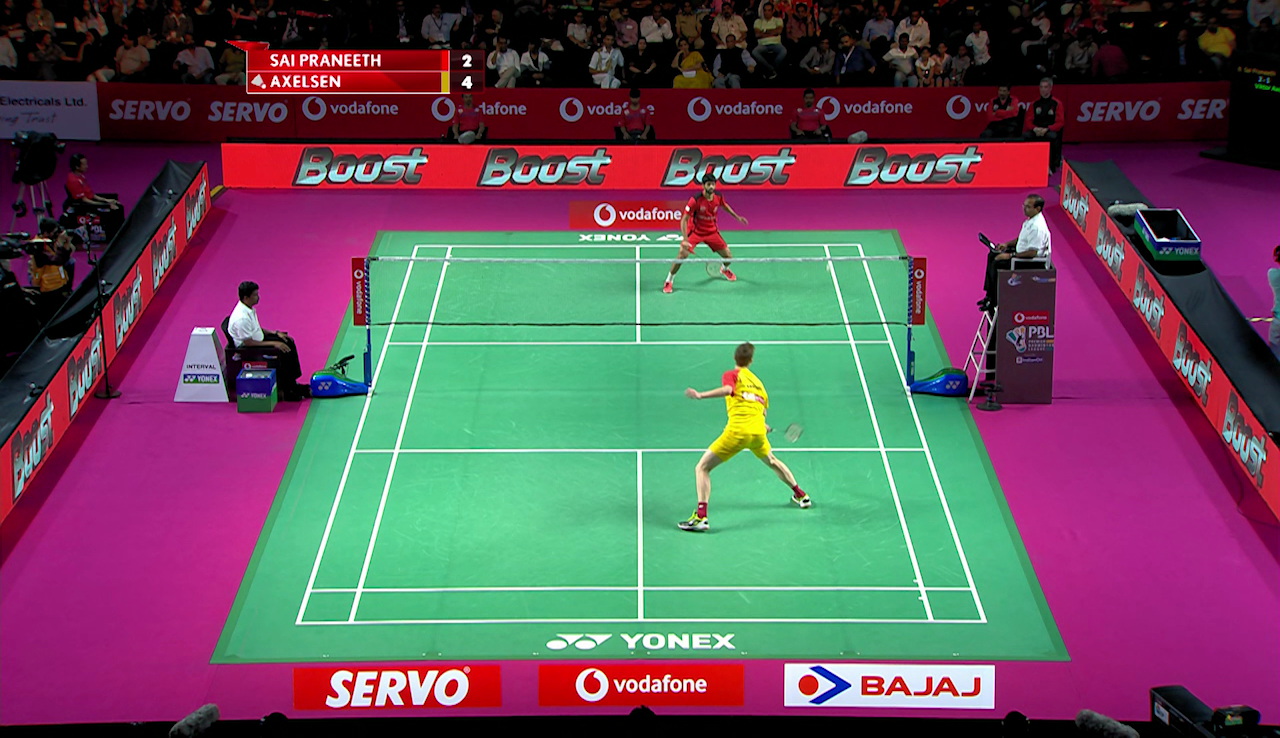
\includegraphics[width=.25\linewidth, height=.2\linewidth]{Images/rally2.png}\hfill
        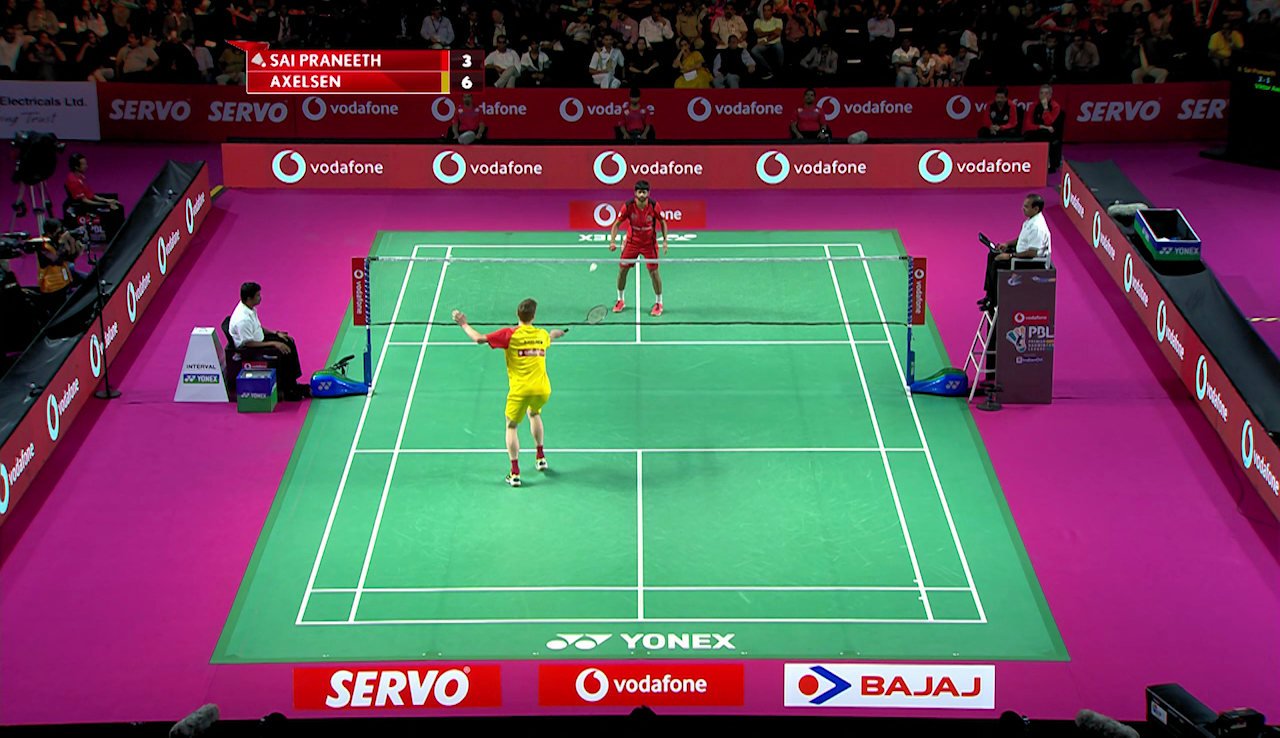
\includegraphics[width=.25\linewidth, height=.2\linewidth]{Images/rally3.png}\hfill
        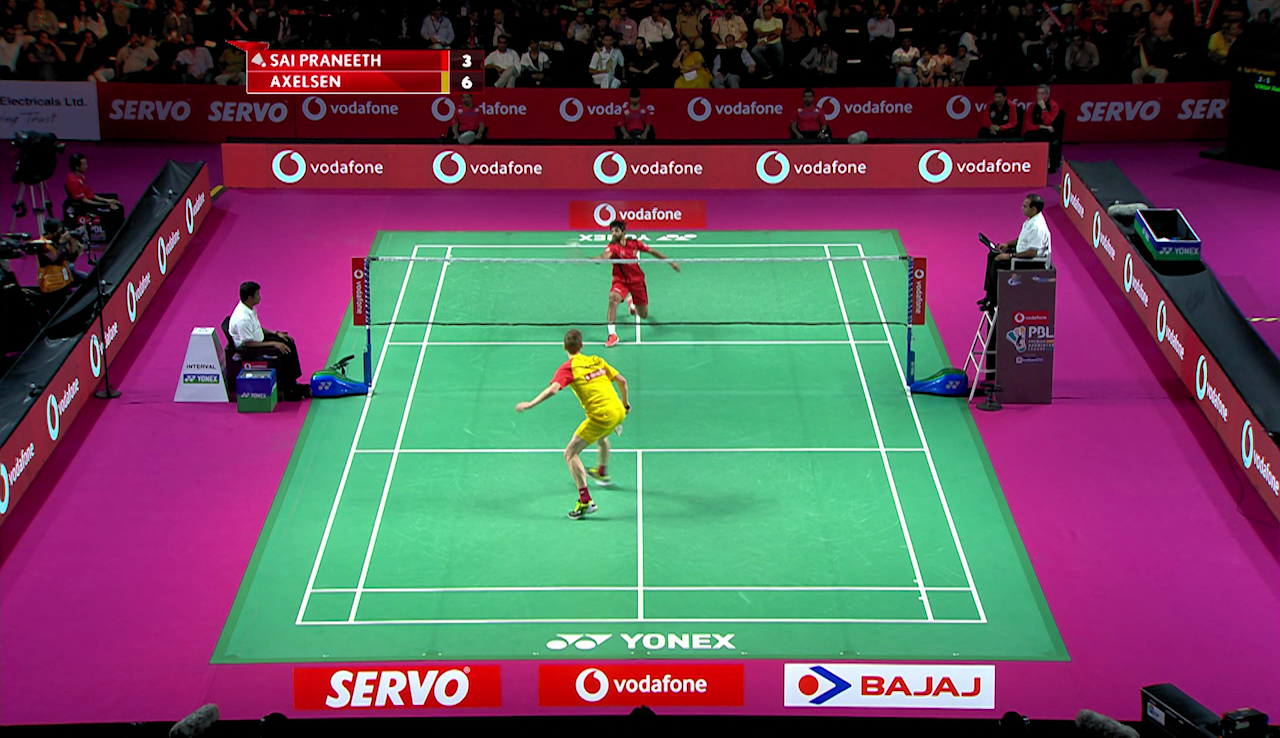
\includegraphics[width=.25\linewidth, height=.2\linewidth]{Images/rally4.png}
        \caption{\label{fig:rallyimg} Rally images output}
    \end{subfigure}\par\medskip
    \begin{subfigure}{\linewidth}
        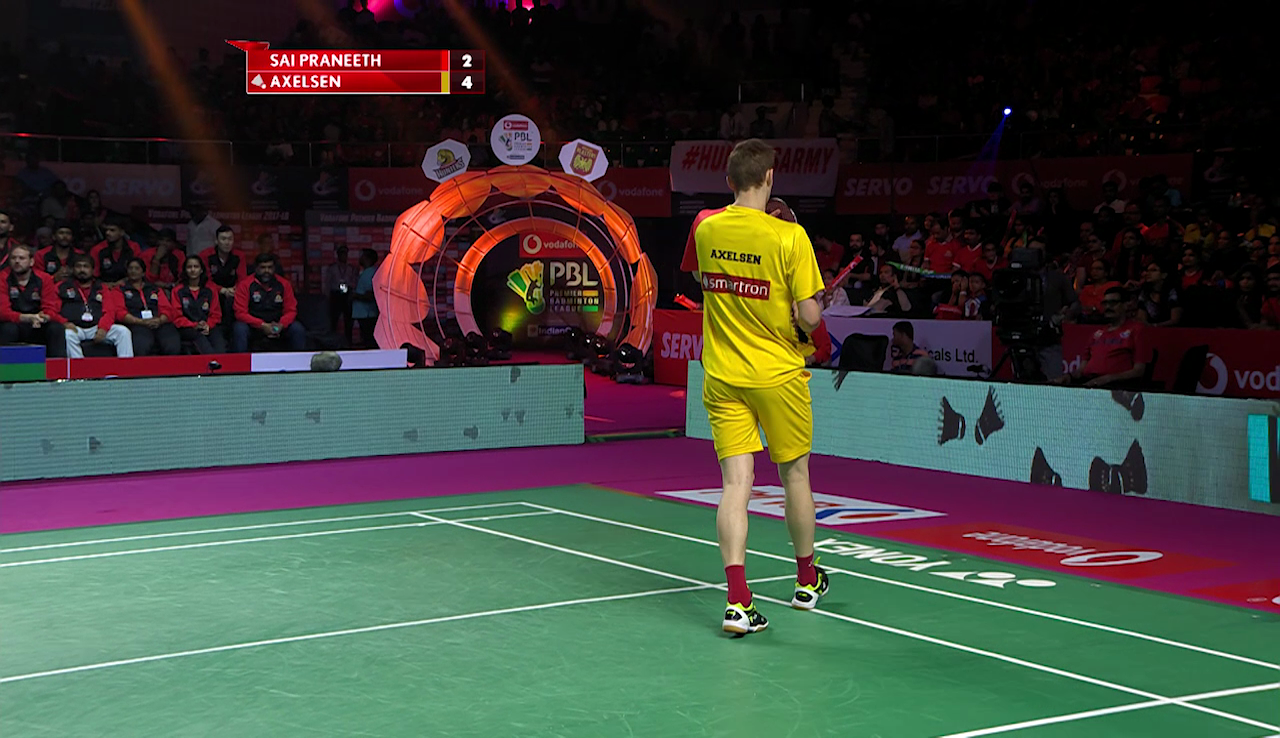
\includegraphics[width=.25\linewidth, height=.2\linewidth]{Images/nonrally1.png}\hfill
        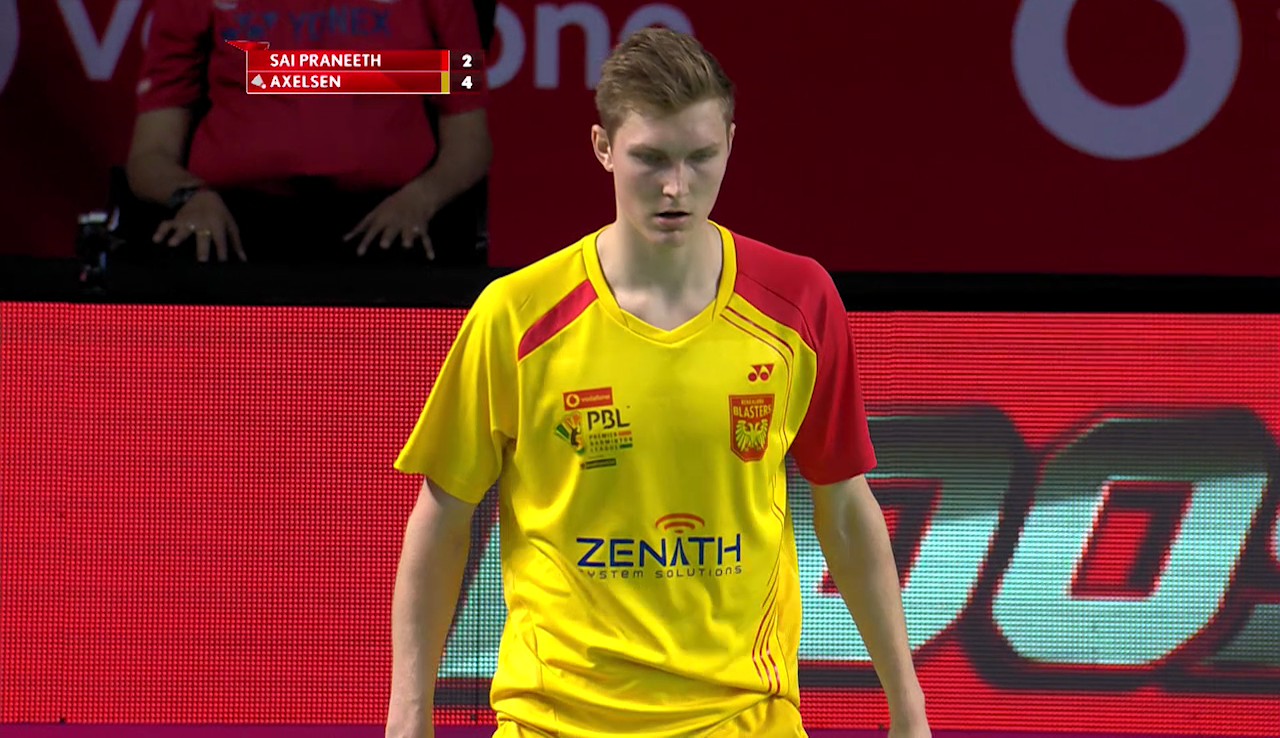
\includegraphics[width=.25\linewidth, height=.2\linewidth]{Images/nonrally2.png}\hfill
        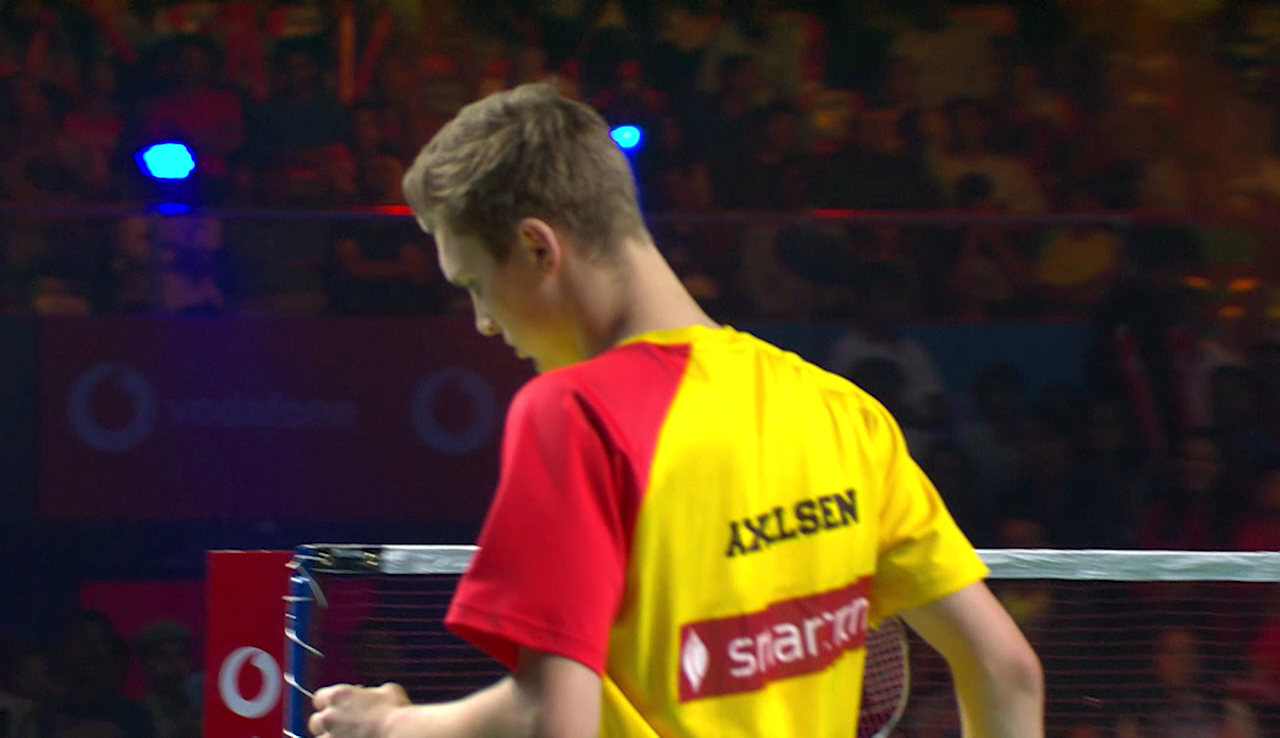
\includegraphics[width=.25\linewidth, height=.2\linewidth]{Images/nonrally3.png}\hfill
        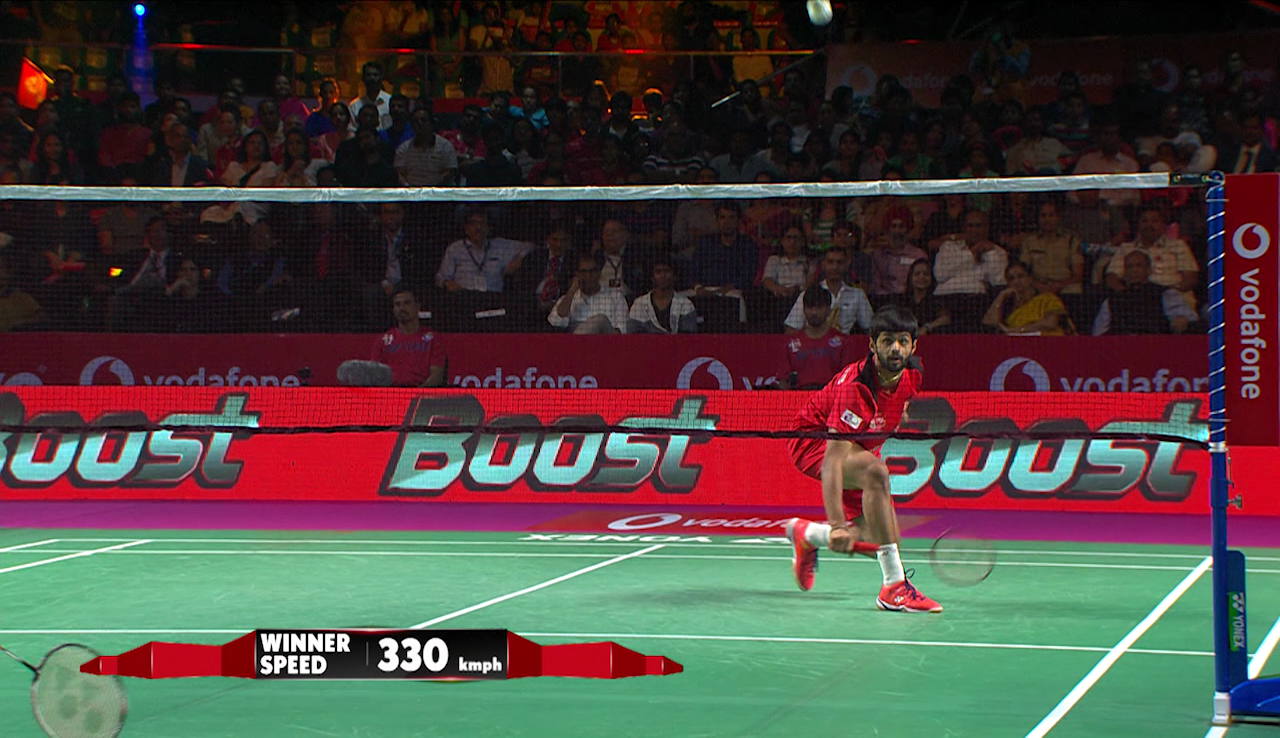
\includegraphics[width=.25\linewidth, height=.2\linewidth]{Images/nonrally4.png}
        \caption{\label{fig:rallyimg} Non-rally images output}
    \end{subfigure}
    \caption{\label{fig:rallynonrally} Output of point segmentation method}
\end{figure}

\subsubsection*{Evaluation:} The average F1 score for the two classes (Rally/Non-Rally) is $97.23\%.$ The precision and recall for the point class are $98.06\%$ and $92.34\%$ respectively.
 
\subsection{Player Tracking and Identification}

We finetune a Faster-RCNN \cite{ren2015faster} network for two classes, "PlayerTop" and "PlayerBottom" with manually annotated players bounding boxes. The "top player" corresponds to the player on the far side of the court and while the bottom player corresponds to the player on the near side of the court w.r.t to the viewpoint of the camera, and we use this notation for brevity. We take each frame from the output of the point segmentation step and obtain the bounding boxes for both the players using the trained model. This approach absolves us from explicitly tracking the players with more complex multi-object trackers.

\begin{figure}[h]
    \centering
    \begin{subfigure}{\linewidth}
        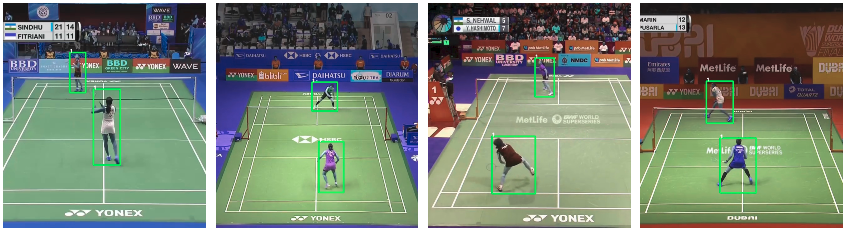
\includegraphics[width=11cm, height=2.5cm]{Images/bb_result.png}
        \caption{\label{fig:bbresultsimple} Output of Faster-RCNN for simple cases}
    \end{subfigure}\par\medskip
    \begin{subfigure}{\linewidth}
        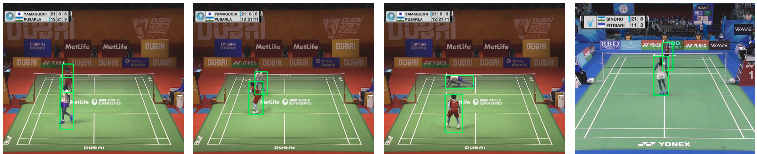
\includegraphics[width=11cm, height=2.5cm]{Images/bb_result_tough.png}
        \caption{\label{fig:bbreulttough} Output of Faster-RCNN for occluded cases}
    \end{subfigure}
    \caption{\label{fig:bbresult} Output of player tracking method. It should be noted that this method is also working fine for tough cases e.g. occlusion and different poses of the player.}
\end{figure}

\subsubsection*{Evaluation:} For evaluating the efficacy of the learned
player detection model, we compute the $\textit{mAP@0.5}$ values on the test set and obtain 99.91\% for overall top and bottom player.

\section{Analyzing points on live match data}

We attempt to extract some meaningful statistics from our data. The temporal structure of Badminton as a sport is characterized by short intermittent actions and high intensity. As we work on live broadcast match videos, we use the above mentioned methodology to get the analysis.

\subsection{Fetching Live Video}

We use the live feed of the broadcast video match from the courtesy of Star Sports India\footnote{https://www.startv.com/about-us/sports/}. We performed our real-time analysis on Premier Badminton League (PBL) - 2019 matches\footnote{http://www.pbl-india.com/}. Generally, the live matches file are growing in nature with time. We retrieve the growing file using FTP server to access for our analysis purposes. We performed each analysis on frame level for the accessed file.
\subsection{Player Bounding Boxes Parallelism}

We perform all the experiment in PyTorch\footnote{https://pytorch.org/} framework for analysis computation. To achieve the analysis in real-time, we used PyTorch's multi-processing library. We fed the output of point segmentation i.e. group of rallies to the multiprocessing library to execute it in a parallel manner. Here is the algorithm used.\\

\begin{algorithm}[H]
\SetAlgoLined
\KwData{Current rally directory}
\KwResult{Player bounding boxes }
 current rally = 1\;
 \If{initial rally is not None}{current rally = initial rally\;}
 \While{True}{
  \If{new rally directory has created}{p = Process(getPlayerBoundingBoxes(current rally))\;
  p.start()\;}
  current rally = current rally + 1\;
 }
 \caption{Multiprocessing to achieve bounding boxes parallelly}
\end{algorithm}

\subsection{Player Distance Calculation}

The player tracks and stroke segments can be utilized in various ways for data analysis. For instance, the simplest method would be the creation of a pictorial point summary. For a given point, we plot the "center bottom" bounding box positions of the player in the top coordinates by computing the homography. This kind of "heatmap" can give us some insights about the particular rally. For example, from figure \ref{fig:heatmap}, it is evident that the bottom player definitely had an upper hand in this point as the top player's positions are scattered around the court. These kind of visualizations are useful to quickly review a match and gain insight into player tactics. \par
We attempt to extract some meaningful statistics from our data. The temporal structure of Badminton as a sport is characterized by short intermittent actions and high intensity. The pace of badminton is swift and the court situation is always continuously evolving, and difficulty of the game is bolstered by the complexity and precision of player movements. The decisive factor for the games is found to be speed and its constituents,
\begin{itemize}
    \item Speed of an individual movement
    \item Frequency of movements
    \item Reaction time
\end{itemize}

In light of such analysis of the badminton game, we define and automatically compute distance covered by both of the players in rallies. To compute the distance covered by the player in a particular rally, we utilize our player tracks. We take the "center bottom" point of the bounding box as a proxy to player current location.

\begin{figure}[!htbp]
    \centering
    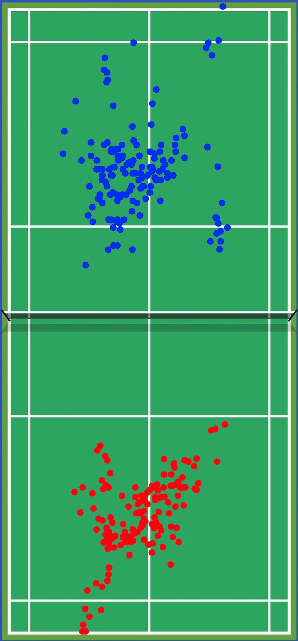
\includegraphics[width=0.8\linewidth]{Images/heatmap.png}
    \caption{\label{fig:heatmap}\textbf{Point Summary:}We show the frame level players’ positions and footwork around the court corresponding to game play of a single point won by the bottom player. Note that, footwork of bottom player is more dense compared to that of top player indicating the dominance of bottom player.}
\end{figure}

\subsubsection*{Top View Space:} We know that displacement of both the players would manifest differently in the camera coordinates. So, using homography techniques we map the 2-dimensional camera co-ordinates to top view court co-ordinates. By doing this, we get a equivalent linear top view space for the player locations. To perform homography calculation, we find the court lines from video frame using Hough line finding method and get the position of court corners. We compute a homography matrix between these court corners and top view court corners to get a mapping from camera co-ordinates to top view space co-ordinates.

\subsubsection*{Distance Calculation:} According to the standard badminton rules\footnote{http://www.worldbadminton.com/rules/}, the length and width of the badminton court for "singles" match is 13.4 mts. and 6.1 mts. respectively. We use this information to find the distance of the player covered in metres. We successively calculate euclidean distance of each frame bounding box for both the players. We scale this pixel based distance into meters to get the actual distance for both the players.
\section{Results}

We now show our result of the analysis which is computed in real-time and got aired in "Hotstar", which is the official Star sports channel. Please refer to the figure \ref{fig:result}. As we do not have any ground truth data for the distance covered by the player, we can't report any accuracy measure here. However, these distances are calculated upon the obtained bounding boxes of the players, we claim that these distances are a good approximation of actual results.
\iftrue
\begin{figure}
    \centering
    \begin{subfigure}{\linewidth}
        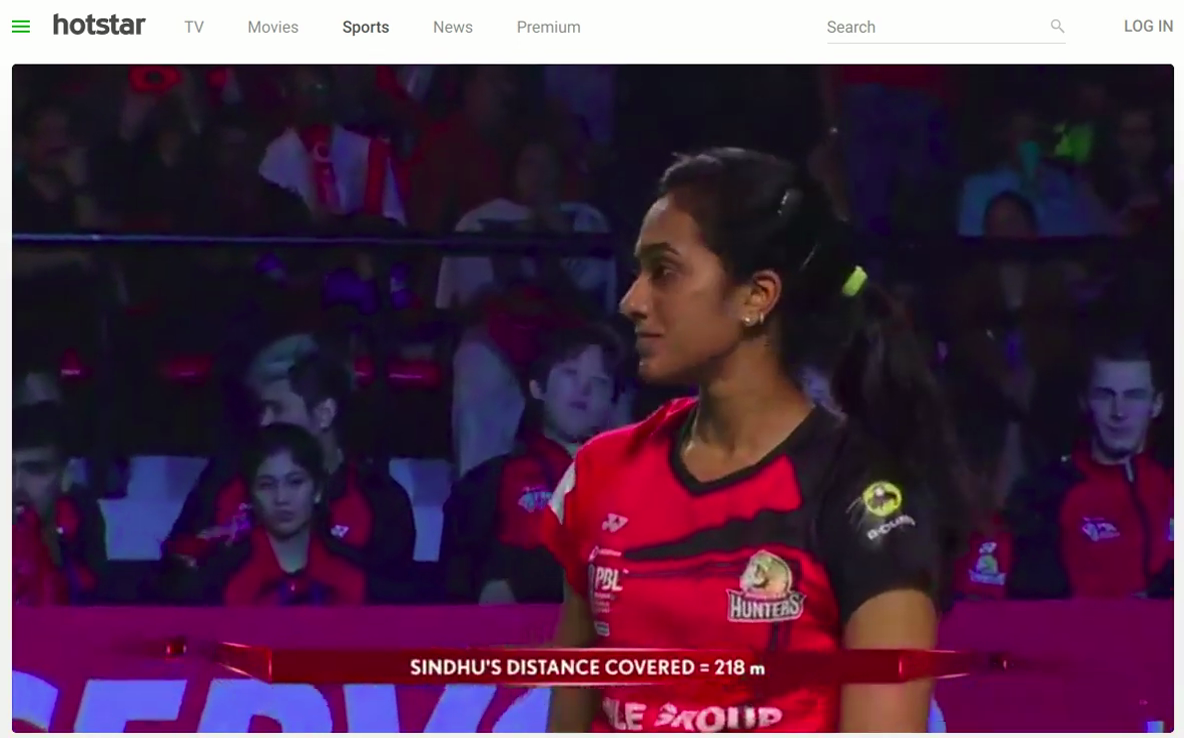
\includegraphics[width=.5\linewidth]{Images/result1.png}\hfill
        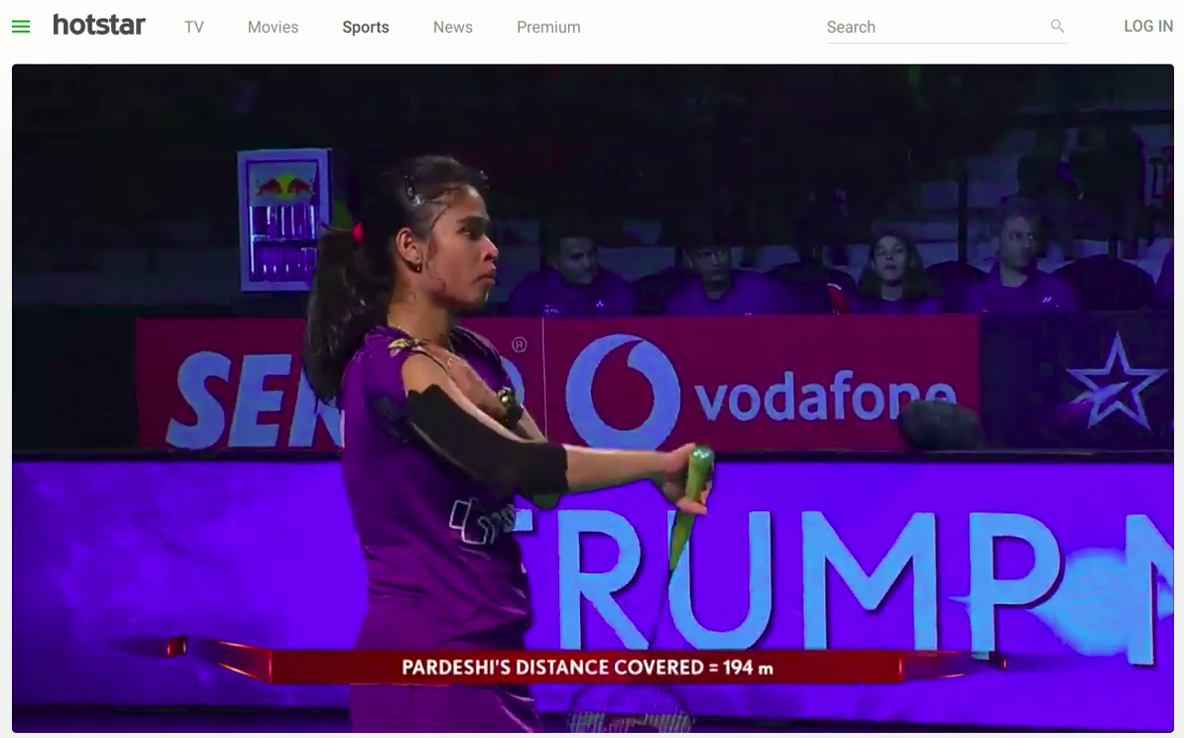
\includegraphics[width=.5\linewidth]{Images/result2.png}\hfill
        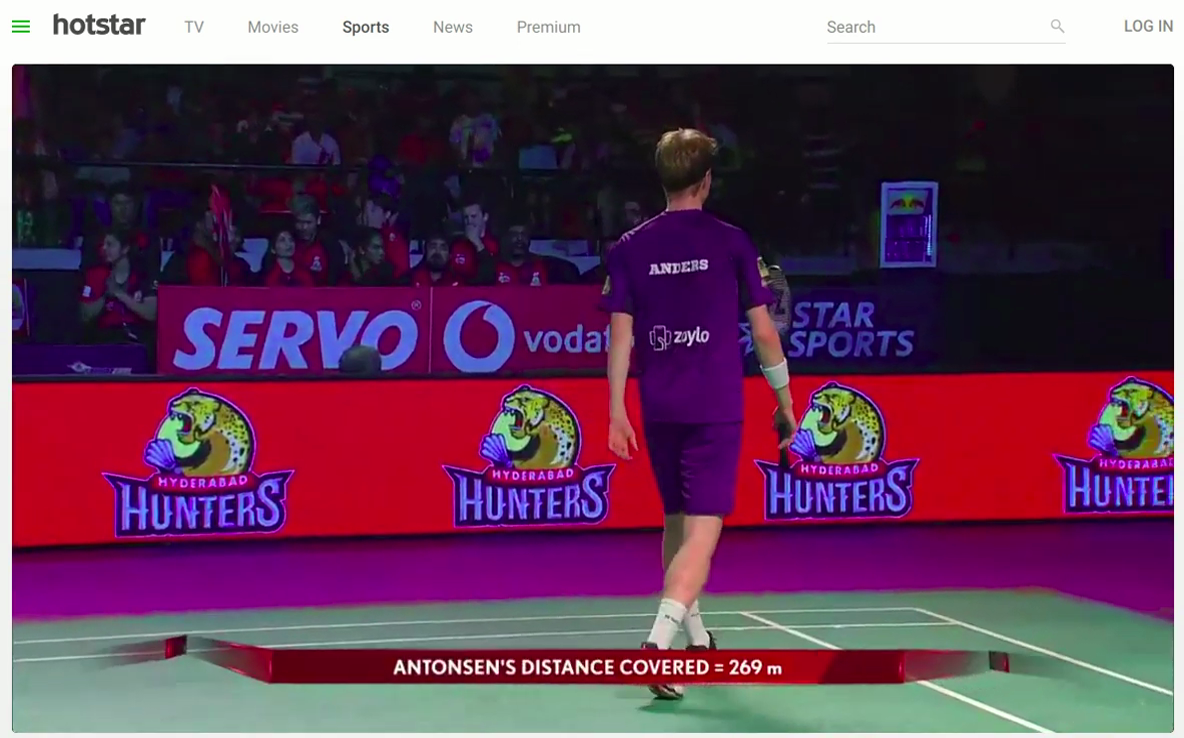
\includegraphics[width=.5\linewidth]{Images/result3.png}\hfill
        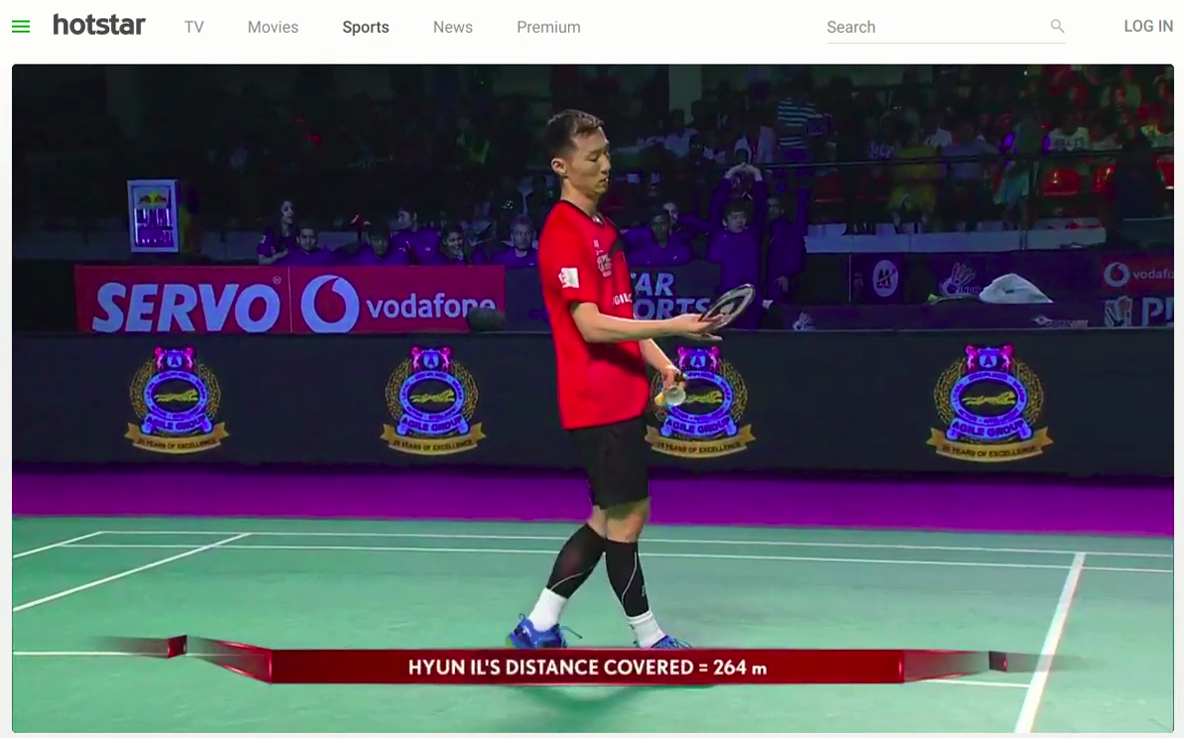
\includegraphics[width=.5\linewidth]{Images/result4.png}\hfill
        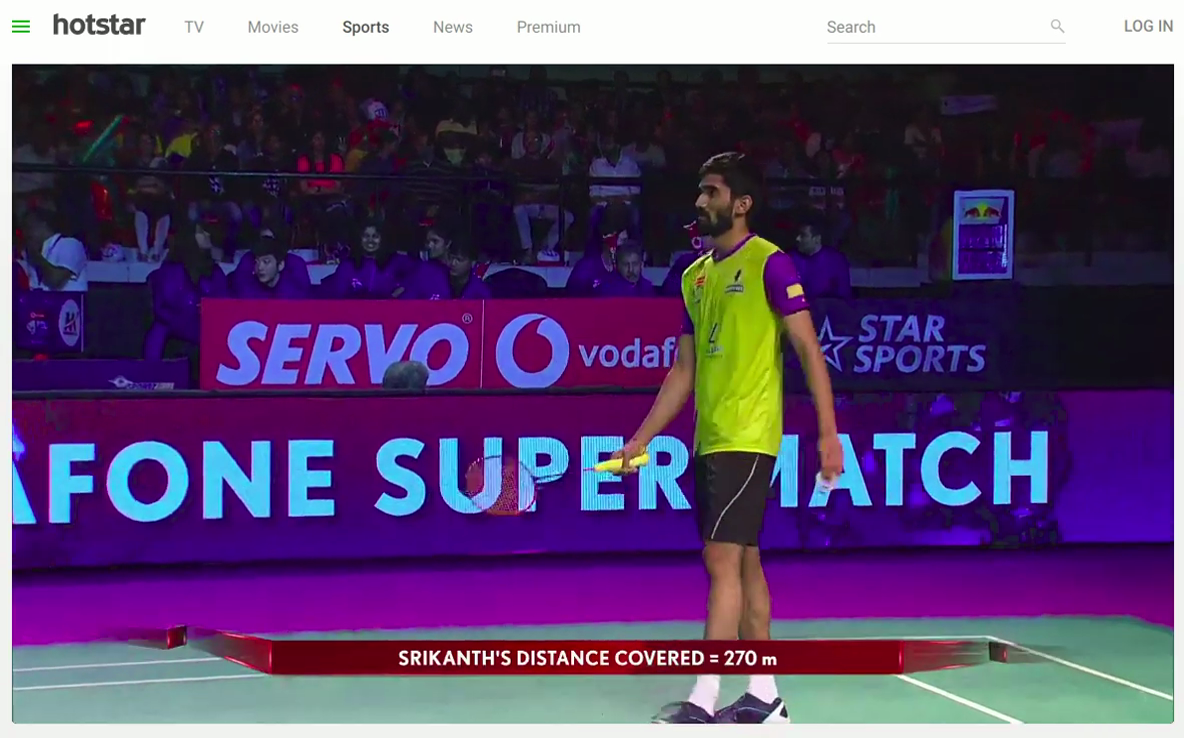
\includegraphics[width=.5\linewidth]{Images/result5.png}\hfill
        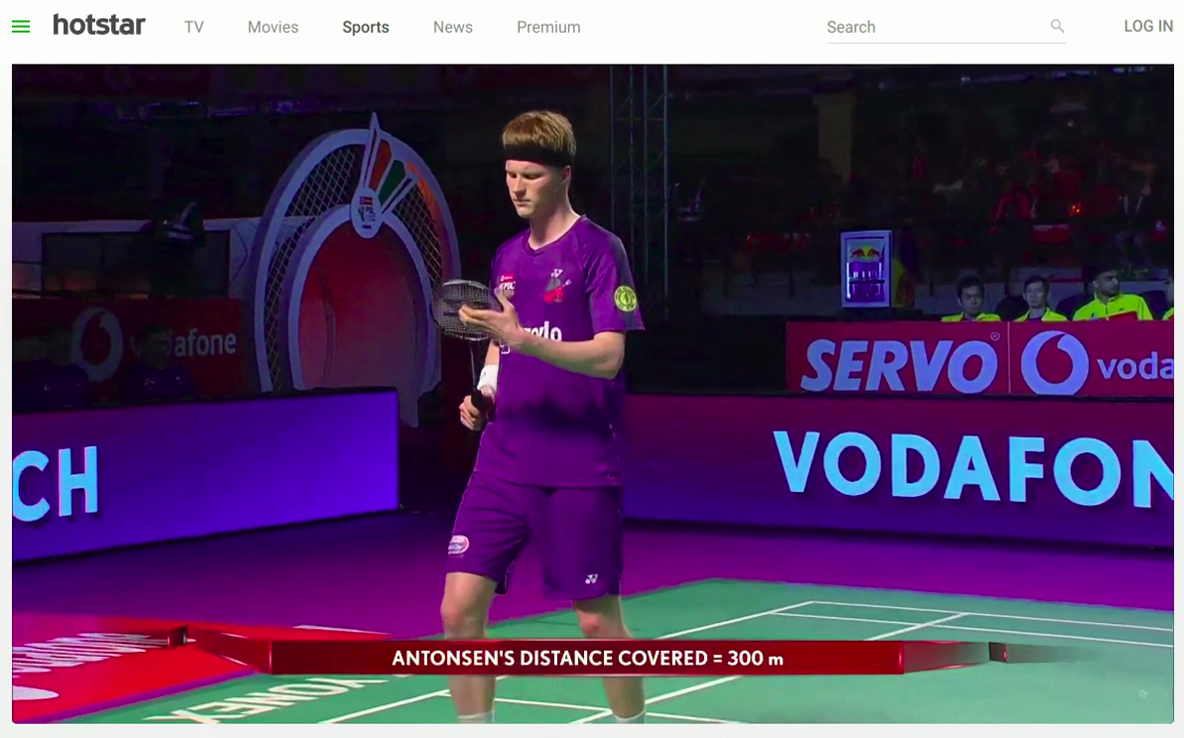
\includegraphics[width=.5\linewidth]{Images/result6.png}\hfill
        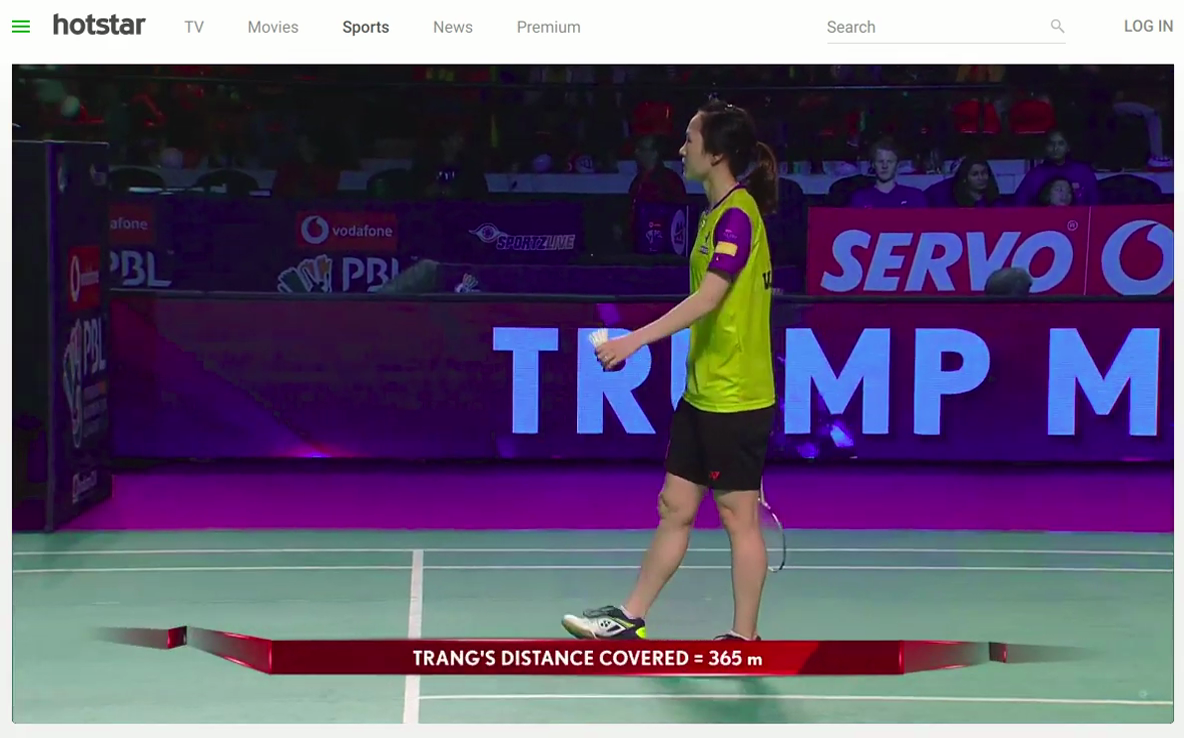
\includegraphics[width=.5\linewidth]{Images/result7.png}\hfill
        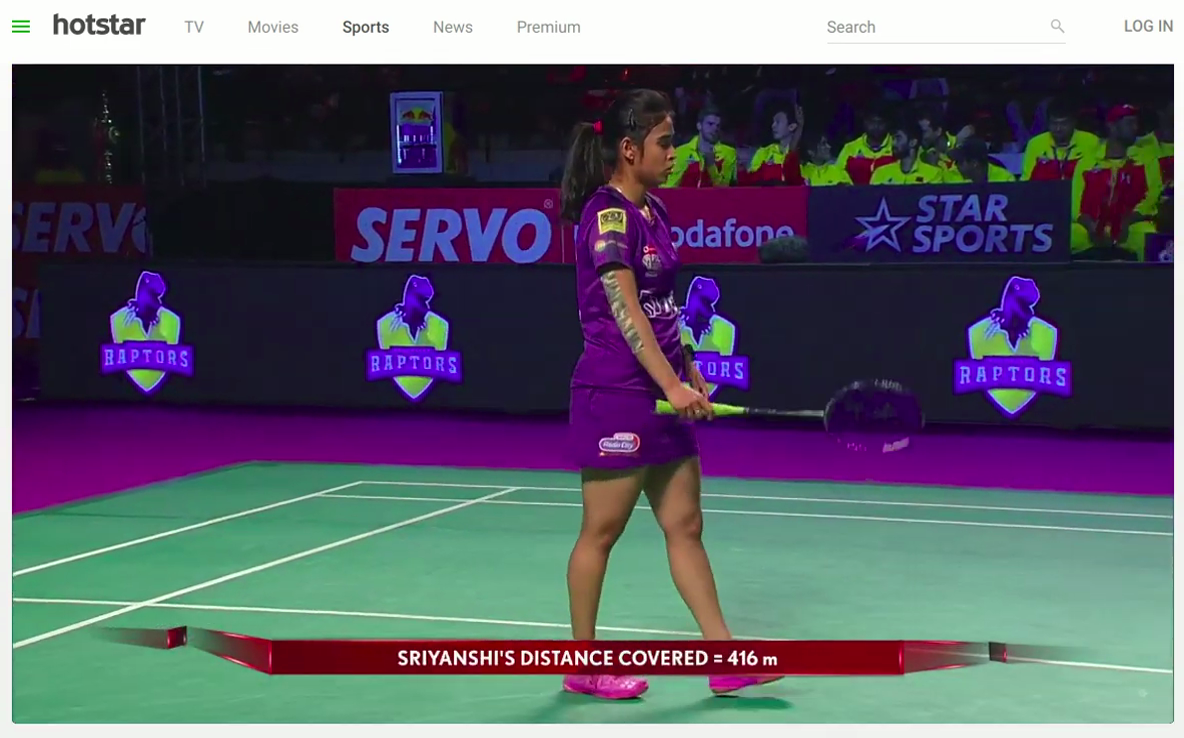
\includegraphics[width=.5\linewidth]{Images/result8.png}
    \end{subfigure}
    \caption{\label{fig:result}The computed player distances for both the players. It should be noted that all results are taken from Hotstar application which confirms the real-time analysis calculation.}
\end{figure}
\fi

\section{Discussion}

In this work, we present an end-to-end framework for automatic analysis of broadcast badminton videos. We build our pipeline on off-the-shelf object detection and homography techniques modules. Analytics for different sports rely on these modules making our pipeline generic for various sports, especially racket sports (tennis, badminton, table tennis, etc.). Although these modules are trained, fine-tuned, and used independently, we could compute various useful as well as easily understandable metrics, from each of these modules, for higher-level analytics. The metrics could be computed or used differently for different sports but the underlying modules rarely change. This is because broadcast videos of different sports share the similar challenges.

\section{Acknowledgment}
We thank Star India Private Limited for providing live feed of the Premier Badminton League - 2019 matches. This work was supported by Product Labs at IIIT-Hyderabad.
\bibliographystyle{plain}
\bibliography{bibliography.bib}
\end{document}
